\documentclass[tikz,border=3pt]{standalone}
\usetikzlibrary{arrows.meta,calc}
\begin{document}
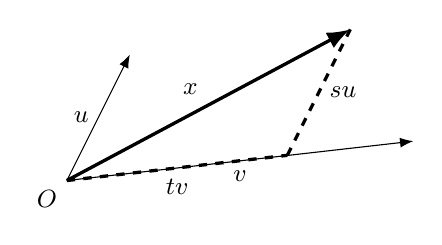
\begin{tikzpicture}[>=Latex, font=\small]
  \coordinate (O) at (0,0);
  \coordinate (U) at (0.8,1.6);
  \coordinate (V) at (4.4,0.5);
  \coordinate (TV) at (2.8,0.32);
  \coordinate (X) at ($(TV)+(U)$);

  \draw[->] (O) -- (V) node[midway, below] {$v$};
  \draw[->] (O) -- (U) node[midway, left] {$u$};

  \draw[dashed, very thick] (O) -- (TV) node[midway, below] {$tv$};
  \draw[dashed, very thick] (TV) -- (X) node[midway, right] {$su$};
  \draw[->, very thick] (O) -- (X) node[midway, above left] {$x$};

  \node[below left] at (O) {$O$};
\end{tikzpicture}
\end{document}
